\documentclass{ITaSconf}
\usepackage[utf8x]{inputenc}
\usepackage[russian]{babel}
\usepackage{url}
\usepackage{xcolor}
\usepackage{graphics}
\usepackage{graphicx}
\usepackage{amssymb}
\usepackage{amsmath}
\usepackage{enumitem}

\usepackage{float}
\floatstyle{plaintop}
\restylefloat{table}

\usepackage{supertabular}

\DeclareMathAlphabet{\mathcal}{OMS}{cmsy}{m}{n}

\newcommand\note[1]{ \textcolor{red}{|| #1 ||} }
\newcommand{\argmin}{\mathop{\rm arg\,min}\limits}
\newcommand{\argmax}{\mathop{\rm arg\,max}\limits}
\def\PP{\mathrm{P}}
\def\RR{\mathbb{R}}
\def\HH{\mathrm{H}}
\def\II{\mathrm{I}}

\title{Выделение пересекающихся сообществ во взвешенных графах на основе методов факторизации матриц}
\author{
  Константин Славнов \\
  \begin{affiliation}
    НИУ ВШЭ
  \end{affiliation}\\
  \email{kaslavnov@edu.hse.ru}
  \and
  Максим Панов \\
  \begin{affiliation}
    НИУ ВШЭ, ИППИ РАН
  \end{affiliation}\\
  \email{panov.maxim@gmail.com}
}

\begin{document}
\maketitle

\begin{abstract}
	В данной работе рассмотрена задача выделения сообществ --- группы вершин в графе, плотно связанных между собой, но не с остальным графом. Известно множество подходов для выделения непересекающихся сообществ \cite{Fortunato10}. Гораздо меньше внимания уделено случаю пересекающихся групп. В работе предложен новый метод решения задачи на взвешенных графах с пересекающимися группами вершин. Метод основан и является обобщением алгоритма BigClam \cite{yang2013overlapping}.
	В конце работы приведены эксперименты. Сравнение с другими методами решения задачи показали, что предложенные алгоритмы работают на уровне современных аналогов, но не лучше их.
	
	Особое внимание уделено методам инициализации BigClam, предложено несколько улучшений, которые ускоряет алгоритм и позволяет сойтись к лучшему значению функции.
\end{abstract}

\textbf{Ключевые слова:} Выделение пересекающихся сообществ, социальные графы, матричное разложение.

\section{Введение}

Сообщества представляют собой основной структурный блок графов реального мира и позволяют понять их структуру и проанализировать свойства.
Целый пласт работ в компьютерных науках, статистике, физике и прикладной математике посвящен выделению структуры сообществ в сложных сетях \cite{Fortunato10}. Сообщество (группа или кластер) интуитивно может быть определено как множество вершин с большим количеством взаимодействий между собой, чем с остальными вершинами графа \cite{girvan2002community}. Такая группа вершин может быть воспринята как структурная единица социальных сетей, либо функциональная в биохимических графах \cite{krogan2006global}, либо как научная дисциплина в сетях цитирования \cite{backstrom2006group}. 

Подобная задача в случае непересекающихся сообществ имеет множество подходов и достаточно подробно изучена \cite{Fortunato10}. Тем не менее, подобные задачи на графах по сих пор активно изучаются. В частности, остаются вопросы как эффективно работать в случае пересекающихся сообществ.
Для решения этой задачи уже разработано несколько методов, например, \cite{airoldi2008mixed}, \cite{palla2005uncovering}, \cite{gregory2010finding}. Однако, проблема остается не до конца изученной. Взвешенные графы представляют дополнительный интерес в этой работе, как более общий случай. Дополнительную сложность составляет отсутствие большого количества данных с верным разбиением на сообщества.

Итак, перейдем к описанию общего подхода к поставленной проблеме и формальной постановке задачи.

\section{Постановка задачи}

Основное предположение, на котором базируется исследование, что чем больше сообществ разделяют две вершины, тем больше вероятность, что они будут соединены ребром. Этот факт находит подтверждение на реальных данных \cite{yang2013overlapping}. Модели, решающие задачу поиска структуры сообществ, должны учитывать этот факт.

В данной работе задача выделения пересекающихся групп вершин будет рассматриваться как некоторая обобщенная проблема матричного разложения. Ее общность заключается в выборе функционала. Критерий качества будет строится исходя из предположений о природе данных. Такой подход позволяет использовать современные наработки по решению оптимизационных проблем такого типа в задаче поиска структуры сообществ.

Представим, что каждая вершина $v$  графа $G$ взаимодействует с сообществом $A$ с некоторой силой $F_{vA}$. Нулевая сила означает отсутствие взаимодействия. Такую модель можно представить как двусвязный граф. Разместим вершины исходного графа $G$ в первой компоненте и вершины-сообщества во второй (рис. \ref{fig:AGM}). Отметим, что подобная концепция позволяет отразить идею не только пересекающихся сообществ, но и вложенных.
\begin{figure}[!ht]
	\centering
	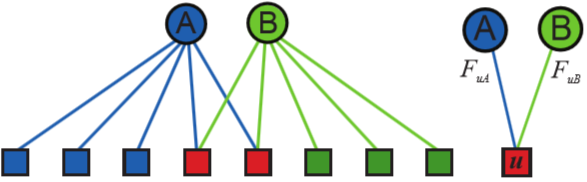
\includegraphics[width=\linewidth]{imgs/BigCLAM_model.png}
	\caption{Двусвязный граф модели BigClam. Сверху вершины-сообщества, снизу вершины исходного графа. Вершины и сообщества взаимодействуют с неотрицательной силой $F_{vA}$. Ребра, которые соответствуют нулевым весам опущены для большей наглядности. \cite{yang2013overlapping}.}
	\label{fig:AGM}
\end{figure}
Определим силу взаимодействия $X_{uv}$ между вершинами $u$ и $v$, которая будет определять вероятность появления ребра между вершинами.
$$X_{uv} = F_{u} \cdot F_{v}^T,$$
где $F_{u}$ --- вектор-строка, составленная из $F_{uA}$ --- сил взаимодействия вершин с сообществами графа.

Таким образом, получено желаемое свойство: чем больше общих сообществ разделяют вершины, тем сильнее они связаны. 
Определим вероятность появления ребра $(u,v)$ как $\PP(u, v) = 1 - \exp ( - X_{uv})$. 
Т.е. чем сильнее связаны вершины, тем вероятнее появление ребра между ними. 
Таким образом получена вероятностная модель. Предполагается, что наблюдаемый нами граф сгенерирован измено из нее.
Позже будет описана вероятностная интерпретация, которая позволит лучше разобраться в описанной модели данных.

Итак, кратко опишем оригинальный метод, его основные предположения.

\subsection{Cluster Affiliation Model for Big Networks (BigClam)}

Введем основные обозначения, которые будут использоваться на протяжении всей работы в Таблице \ref{table:notation}. 
\begin{table}[!t]
	{
	\centering
	\small
	\begin{tabular}{ p{5.5em}   p{17.5em} }
		\hline
		\hline
		Обозначение 						& Описание \\
		\hline
		$G = (V,E) $ 						& граф \\             
		$N$    								& количество вершин в графе \\  
		$K$    								& количество сообществ \\      
		$A \in \mathbb{R}_{+}^{N\times N}$  & матрица смежности   \\
		$F \in \mathbb{R}_{+}^{N\times K}$  & матрица силы принадлежности к сообществам			\\
		$C$    								& множество сообществ  \\
		$\PP(u,v)$							& вероятность появления ребра $(u,v)$ \\
		$\PP((u,v) \mid c)$ 					& вероятность появления ребра $(u,v)$ при условии, что $u$ и $v$ принадлежат сообществу $c$ \\
		
		$l(F)$								& логарифм функции правдоподобия \\
		$\mathcal{N}(u)$ 					& 1-окрестность вершины $u$ (cоседи вершины) \\
		$w_{uv}$							& вес ребра $(u,v)$ для взвешенного графа \\
		\hline
		\hline
	\end{tabular}
	}
	\caption{Основные обозначения работы.}
	\label{table:notation}
\end{table}
Рассмотрим следующие предположения, которые лежат в основе всей модели.
\begin{enumerate}
	\item Каждая вершина $v\in V$ относится к сообществу $c \in C$ с некоторой силой
	$F_{vc} \ge 0.$
	\item Вероятность появления ребра $(u,v)$, при условии, что вершины $u,v$ находятся в одном сообществе $c$ определяется по формуле 
	$$\PP((u,v) \mid c)=1 - \exp(-F_{uc}\cdot F_{vc}).$$
	\item Каждое сообщество $c$ генерирует ребра независимо от других, а значит, что вероятность появления ребра можно посчитать по формуле для независимых случайных величин. Получим
	$$\PP(u,v)=1 - \exp(-\sum_{c\in C} F_{uc} F_{vc}) = 1 - \exp( - F_{u} F_{v}^T),$$
	$$F = \{F_u\} = \{F_{uc}\} \in \mathbb {R}^{N \times K}. $$
\end{enumerate}

Предложенная модель имеет простую вероятностную интерпретацию. 
Предположим, что существуют скрытые случайные переменные $X_{uv}$, которые определяют силу взаимодействия вершин, а ребро появляется, если  $X_{uv} > 0$.
Каждое сообщество графа дает свой независимый вклад $X_{uv}^{(c)}$ в $X_{uv}$.
Предположим, что $X_{uv}^{(c)} \sim \mathrm{Pois}(F_{uc} \cdot F_{vc})$, где $F_{vc}\ge 0$ сила взаимодействия вершины $v$ и сообщества $c$. 
Значит, что 
$$X_{uv} \sim \mathrm{Pois}(\sum_{c} F_{uc} \cdot F_{vc}) = \mathrm{Pois}(F_{u} \cdot F_{v}^T).$$
Вероятность появления ребра равна 
$$p(u,v) = \PP(X_{uv} > 0) = 1 - \exp( - F_{u} F_{v}^T),$$
что соответствует формулам, полученным выше.

Для восстановления матрицы $F$ предлагается использовать метод максимизации правдоподобия.
Из приведенных выше формул не сложно вывести, что правдоподобие $l(F)$ определяется как
\begin{flalign*}
	l(F) & = \log(\PP(A\mid F)) \\
		 & = \sum_{(u,v)\in E} \log(1 - \exp( - F_{u} F_{v}^T)) - \sum_{(u,v) \notin E} F_u F_v^T.
\end{flalign*}

Для оптимизации возьмем алгоритм блочного координатного спуска с методом проекции градиента на каждом шаге.
Фиксируется значение $F_v$, оптимизация ведется по $F_u$, $u \ne v$. Задача становится выпуклой и может быть сформулирована как
$$\forall u: \quad \argmax_{F_u \ge 0} l(F_u), $$
где 
$\displaystyle l(F_u) = \sum_{v \in \mathcal{N}(u)} \log(1-\exp(-F_u F_v^T)) - \sum_{v \notin \mathcal{N}(u)} F_u F_v^T, $
$\mathcal{N}(u)$ — соседи вершины u.

Несложно убедиться, что градиент такого функционала может быть вычислен как
$$\nabla l(F_u) = \sum_{v \in \mathcal{N}(u)} F_u \dfrac{\exp(-F_u F_v^T)}{1-\exp(-F_u F_v^T)} - \sum_{v \notin \mathcal{N}(u)} F_v^T. $$

Основная сложность формулы (линейная по размеру графа) сконцентрирована во втором слагаемом. Заметим, что 
$$\sum_{v \notin \mathcal{N}(u)} F_v^T = \sum_v{F_v} - F_u - \sum_{v\in \mathcal{N}(u)} F_v.$$ 
Значение $\sum_v{F_v}$ легко поддерживать в памяти, обновляя на каждой итерации за константное время. Получаем сложность одной итерации $O(\mathcal{N}(u))$. 
В этом заключается значимое отличие рассматриваемого метода. 
Такая сложность позволяет обсчитывать графы с количеством вершин до $10^5$ за приемлемое время.

Для подбора градиентного шага используется backtracking line search \cite{boyd2004convex}.

Опишем связь данной задачи с матричными разложениями.
Подобная постановка задачи позволяет рассмотреть задачу выделения пересекающися сообществ как задачу неотрицательного матричного разложения с общим функционалом.
То есть, необходимо найти такую низкоранговую матрицу $F\in \mathbb{R}_{+}^{N \times K}$, что она наилучшим образом приближает значение $A$ в смысле некоторого функционала:
$$ F = \argmin_{F\ge 0} D(A, f(F F^T)). $$

В качестве меры ошибки между матрицей и ее аппроксимацией выступает функция $D(\cdot, f(\cdot))$. В нашем случае
$D = -l(F)$ --- значение правдоподобия, а $f(x) = 1 - \exp(-x)$ --- функция, которая преобразует силы взаимодействия вершин в вероятности появления ребра (link function). Эта часть функционала делает его более пригодным к анализу бинарных матриц, чем стандартная $l_2$-норма.

Поэтому в качестве оптимизационной схемы берется стандартный метод для решения задач матричного разложения \cite{lin2007projected}.

После того, как метод оптимизации сошелся к некоторому оптимальному значению матрицы, осталось перейти к задаче выделения групп вершин по $F$.
Для того, чтобы восстановить исходную структуру сообществ $C$, сравним значение матрицы $F$ с некоторым порогом $\delta$. Если $F_{vc} > \delta$, то $v \in c$. $\delta$ выберем следующим образом.

Обозначим за $\varepsilon$ вероятность появления ребра в графе (если бы все ребра появлялись равномерно): 
$$\varepsilon = \dfrac{2|V|}{|E|\cdot (|E|-1)}.$$ 
Возьмем $\delta$ так, чтобы две вершины принадлежали одному сообществу, если модельная вероятность появления ребра между ними выше чем $\varepsilon$:
$$\varepsilon \le 1-\exp(-\delta^2).$$
А значит
$$\delta = \sqrt{-\log(1-\varepsilon)}. $$

Описанный метод обладает одним незначительным недостатком.
Если две вершины не разделяют хотя бы одного общего сообщества, между ними не может быть ребра.  
Очевидно, что в настоящих сетях такого свойства нет.
Поэтому введем так называемое $\varepsilon$-сообщество.
Предполагаем, что все вершины относятся к единому $\varepsilon$-сообществу с малой силой $\delta$, определенной выше.
То есть дополнительно предполагается, что ребро могло возникнуть случайно с вероятностью, которая равна доле существующих ребрер в графе:
$$ \PP((u,v)\mid \varepsilon) = \dfrac{2|V|}{|E| \cdot \left( |E| - 1 \right)}.$$

\section{Инициализация}

В предыдущем разделе был полностью описан метод BigClam зи исключением способа инициализации. 
Так как задача не является выпуклой, большое внимание необходимо уделить этому аспекту. 
В ходе анализа было замечено, что метод подбора начального приближения матрицы $F$ можно усовершенствовать. 
Все результаты и наблюдения будут подробно описаны в этой части работы. 
Начнем с описания оригинального метода инициализации из статьи \cite{gleich2011neighborhoods}. 

\subsection{Оригинальный подход}

Введем метрику на подмножестве множества вершин $ S \subset V $.
$$\phi(S) = \dfrac{\mathrm{cut}(S)}{\min(\mathrm{vol}(S), \mathrm{vol}( \bar S))},$$
где $\mathrm{cut}(S)$ --- разрез подмножества $S$, $\mathrm{vol}(S)$ --- его объем:
$$\mathrm{cut}(S) = \mathrm{cut}(S, \bar S)=\sum_{\substack{(v,u)\in E\\ v \in S \, u \in \bar S}} a_{vu},$$
$$\mathrm{vol}(S) =\sum_{\substack{(v,u)\in E,\\ v \in S}} a_{vu}.$$

Величина $\phi(S)$ называется проводимостью (conductance) и очень похожа на взвешенный разрез.
Утверждается, что эго-графы (вершина с ее 1-окрестностью), которые достигают локального значения функционала $\phi(S)$,  являются хорошими сообществами и могут использоваться в качестве инициализации для других методов \cite{gleich2011neighborhoods}.
Локальность понимается в смысле локальности на графе. 
То есть значение проводимости эго-графа любой соседней вершины должно быть больше, чем в данной. 

В качестве инициализации предлагается выбрать необходимое количество эго-графов, которые достигают локального минимума. Если таких графов больше, чем требуется, выберем те, у которых минимальное значение проводимости.
То есть для 
$$S_1 \equiv \mathcal{N}(v_1), \dots, S_K \equiv \mathcal{N}(v_K)\,:\:\phi(S_1) \le \cdots \le \phi(S_K),$$
$v_i \in V$ --- вершины локального минимума: $\forall u \in \mathcal{N}(v_i) \, : \: \phi(\mathcal{N}(u)) > \phi(\mathcal{N}(v_i))$,
$$ 
F_{ij}=	
\begin{cases} 	1,  \text{если } v_i \in S_j;\\
0,  \text{иначе. } 
\end{cases}
$$
Если $S_i$ меньше необходимого числа, заполним остальные столбцы матрицы случайным образом.

Опишем минусы такого подхода. 
Матрица $F$ получается детерминированной, а значит нельзя перезапускать метод для поиска лучшего результата.
$F$ состоит всего из двух значений 0 и 1, при чем подавляющее большинство нули. 
Ноль является плохой точкой для старта, т.к. $F=0$ --- точка локального минимума и модель потенциально может сойтись к плохому значению функционала.
Помимо этого, часто так получается, что 2 или более значений среди $S_1, \dots, S_K$ соответствуют одному сообществу. 
Продемонстрируем последний недостаток на следующем модельном примере.

Рассмотрим матрицу $F\in \RR_{+}^{3\times 140}$ как на рис. \ref{fig:model_ex}. 
Сгенерируем из нее модельный граф согласно модели BigClam. 
Найдем 3 вершины, эго-графы которых будут образовывать начальное приближение матрицы $F$. 
На рис. \ref{fig:model_ex_graph} изображен семплированный граф. 
На левой части красным цветом отмечены 3 найденные вершины.
\begin{figure}[!ht]
	\centering
	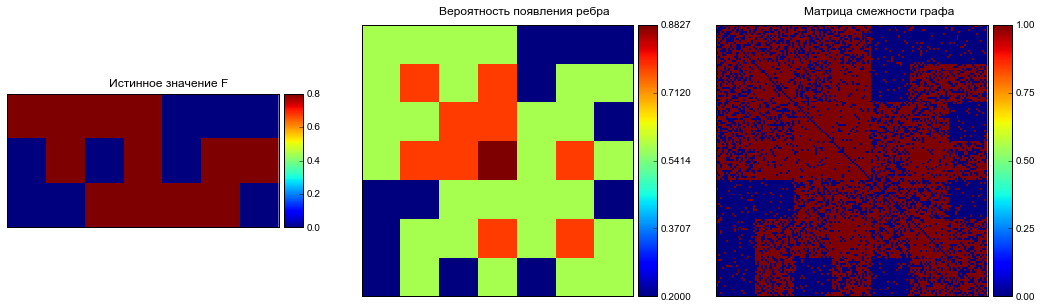
\includegraphics[width=\linewidth]{imgs/model_example.png}
	\caption{Модельный пример графа с 140 вершинами и тремя пересекающимися сообществами. Cлева матрица $F$; по середине матрица вероятностей появления ребра $1-\exp(FF^T)$; \textbf{справа} случайная семплированная матрица смежности.}
	\label{fig:model_ex}
\end{figure}
\begin{figure}[!ht]
	\centering
	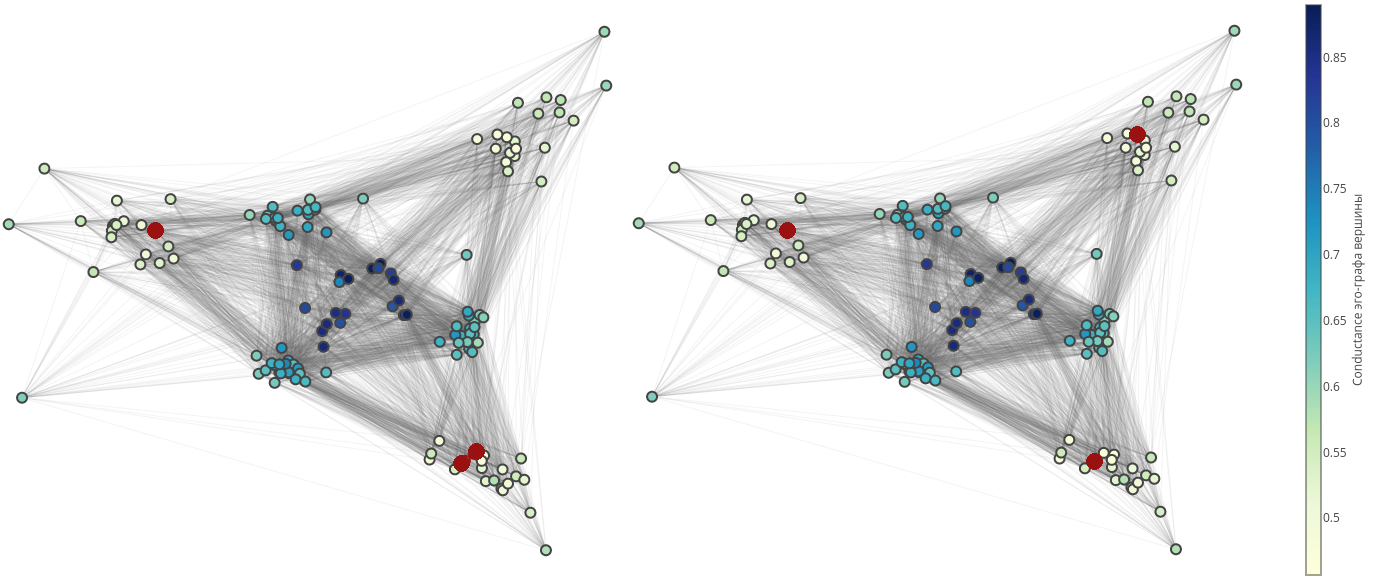
\includegraphics[width=\linewidth]{imgs/model_example_graph_good_init_pres.png}
	\caption{Граф, сгенерированный из матрицы $F$ на рис. \ref{fig:model_ex}. Красным цветом обозначены вершины, эго-графы которых образуют начальное приближение матрицы $F$. \textbf{Слева} оригинальный метод. Две вершины попали в один кластер, что портит начальное приближение. \textbf{Справа} новый метод. Все 3 вершины лежат в своих кластерах, что улучшает качество инициализации.}
	\label{fig:model_ex_graph}
\end{figure}
Видно, что 2 вершины являются представителями одного и того же сообщества. 
И это не единичный случай, такая ситуация часто встречалась в том числе на реальных графах. 


Формально, можно сказать, что часто находятся такие $i,j \in {1,\dots, K}$, что ${F_{\bullet i}}^T F_{\bullet j} \gg 0$, где $F_{\bullet i} = \{F_{j i}\}_{j=1}^N$, а значит эго-графы вершин значительно пересекаются. 
Вершины лежат рядом, и велика вероятность того, что принадлежат к одному и тому же сообществу.

\subsection{Новый подход}

Решением описанной выше проблемы может послужить дополнительная регуляризация за близкое расположение к уже взятым в качестве инициализации вершинам. 
То есть при инициализации следующего вектор-столбца $F_{\bullet j}$, добавим штраф к значению проводимости $S_i$ эго-графа $i$ вершины. Штраф положим равным 
$R = \gamma \cdot {F_{\mathrm{s}}}^T  F_{\mathrm{e}_i},$
где $F_{\mathrm{s}, l} = 1$ в вершинах, которые уже входят в инициализацию ( $\exists k:\, F_{lk}=1 $),
а $F_{\mathrm{e}_i, l} = 1$, если $l$ лежит в эго-графе $i$ вершины ($l \in \mathcal{N}(i)$),
$\gamma = 1 / \sum_l F_{\mathrm{s}, l}$ --- нормировка. 
То есть $R$ --- доля уже выбранных вершин, которые попали в рассматриваемый эго-граф.  

Результат работы метода на текущем примере отражен на правой части рис. \ref{fig:model_ex_graph}. Желаемый результат достигнут. Для большей общности можно было бы ввести коэффициент регуляризации, но было решено этого не делать и учитывать 2 критерия (проводимость и коррелированность) с одинаковым весом. 

Таким образом получилось избавиться от одной описанной выше проблемы. 
Проблема нулей и детерминированности решается простым добавлением равномерного шума в диапазоне $[0; 0.1]$. Константа $0.1$ подобрана экспериментально. 

Дополнительно возникла идея, что вершины соседние к эго-графу имеют большую вероятность принадлежать к тому же сообществу, чем остальные. 
Значит вокруг найденного начального приближения можно ``распространить''  его на соседние вершины. 
То есть дать половину веса (0.5) всем вершинам, соседним к найденному эго-графу.
\begin{center}
	\begin{table*}
		\centering
		\begin{tabular}{ p{9.5em}   p{38em} }
			\hline
			\hline
			\textbf{Обозначение} 		& \textbf{Описание} \\
			\hline
			\textit{rand} 				& Инициализация равномерным шумом от 0.75 до 1.25 \\
			\textit{cond} 				& Инициализация в локальных максимумах проводимости (стандартный метод) \\
			\textit{cond\_new} 			& Новый метод со штрафом за пересечение с уже выбранными вершинами \\
			\textit{cond\_randz} 		& Дополнительно заменяем нули из метода \textit{cond} на значения от 0 до 0.1 \\
			\textit{cond\_new\_randz} 	& Дополнительно заменяем нули из метода \textit{cond\_new} на значения от 0 до 0.1 \\
			\textit{cond\_randz\_spr} 	& Применяем метод \textit{cond}. Соседние с найденными эго-графами вершины получают половину его веса. Затем заменяем нули матрицы $F$ на значения от 0 до 0.1 \\
			\textit{cond\_new\_randz\_spr} & Применяем метод \textit{cond\_new}. Соседние с найденными сообществами вершины получают половину его веса. Затем заменяем нули матрицы $F$ на значения от 0 до 0.1 \\
			\hline
			\hline
		\end{tabular}
		\caption{Расшифровка обозначений для методов инициализации.}
		\label{table:init_methods}
	\end{table*}
\end{center}
\subsection{Эксперименты} 

По итогам исследования появилось целое семейство методов инициализации. 
В ходе экспериментов было изучено поведение правдоподобия на модельных и реальных данных. 
Эксперименты проводились на модели данных, предложенной в \cite{lancichinetti2009benchmarks}. 
Таблица \ref{table:bench_params} содержит используемые для генерации параметры. 
О модели и ее параметрах речь пойдет позже, в секции посвященной основным экспериментам данной работы.

В качестве реальных графов взяты 4 эго-графа (граф знакомств друзей конкретного человека) из социальной сети ``В Контакте''.

В Таблице \ref{table:init_methods} приведено описание исследуемых методов инициализации.
На рис. \ref{fig:llh_init_model} и \ref{fig:llh_init_real} показано поведение правдоподобия в зависимости от номера итерации для модельных и реальных данных соотвественно.
 
\begin{figure}[!h]
	\centering
	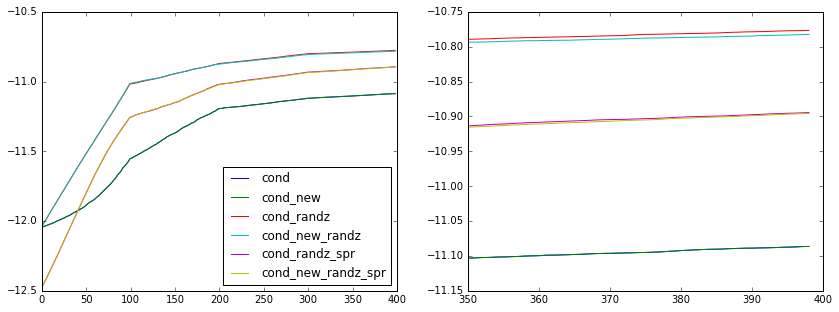
\includegraphics[width=\linewidth]{imgs/init_new_good.png}
	\caption{Поведение двойного логарифма правдоподобия (ось y) в зависимости от номера итерации (ось х) для различных начальных приближений для модельных данных \cite{lancichinetti2009benchmarks} с 1000 вершинами. Было произведено усреднение по 50 графам. Справа показано завершение оптимизации. Видно, что добавление случайного шума значительно улучшает итоговый результат, в то время как метод со штрафом не существенно отличается от оригинального.}
	\label{fig:llh_init_model}
\end{figure}
\begin{figure}[!h]
	\centering
	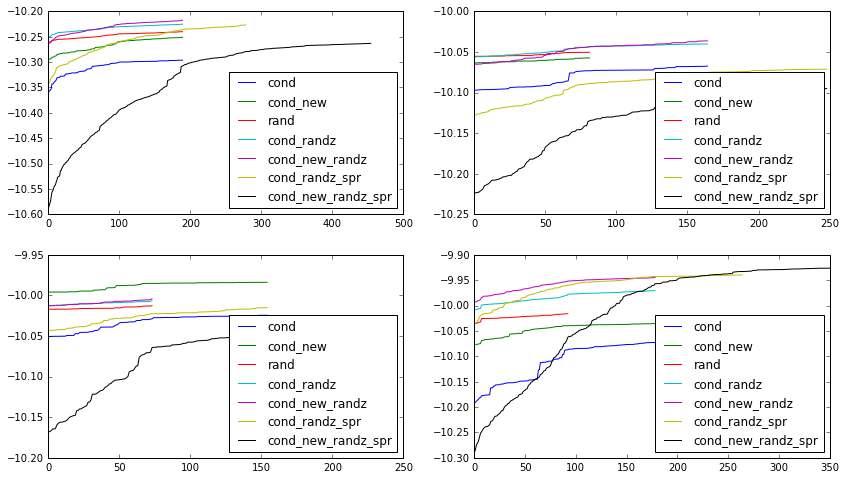
\includegraphics[width=\linewidth]{imgs/init_llh_real.png}
	\caption{Поведение двойного логарифма правдоподобия (ось y) в зависимости от номера итерации (ось х) для различных начальных приближений для четырех реальных графов (4 графика). Показано завершение оптимизации и 0 по горизонтальной оси соответствует 250 итерации. В трех случаях лидируют новые методы, в одном лидирует случайная инициализация, но проигрывает по временным затратам. }
	\label{fig:llh_init_real}
\end{figure}
\subsection{Выводы} 
По итогам тестов можно сказать, что предложенные методы инициализации демонстрируют лучший результат. 
Начальные приближения оказались лучше по правдоподобию, как следствие, метод сходится быстрее и к немного лучшим значениям функционала. 
На модельных данных основное улучшение достигнуто путем добавления равномерного шума, и идея со штрафом не проявила себя.

На реальных данных преимущества нового подхода с регуляризацией очевидно. 
Похоже, что старая инициализация приводит к плохим локальным максимумам. 
Идея же с распространением (методы с приставкой \textit{\_spr}) не оправдалась и как минимум нуждается в дополнительной проверке.

\section{Модели для взвешенных графов}

Перейдем к основной теме данной работы: выделение пересекающихся сообществ в взвешенном графе. 
Такие методы полезны тем, что позволят учесть дополнительную информацию, которая часто дополняет матрицу смежности, но не может напрямую использоваться в методах, работающих с бинарной матрицей смежности, как BigClam.

Начнем с самого простого и интуитивного обобщения метода BigClam, который будем называть наивный взвешенный BigClam.
Вес ребра $(u,v)$ обозначим за $w_{uv}$. 
Для обработки взвешенных ребер изменим функционал качества следующим образом:
$$l(F) = \sum_{(u,v)\in E} \log\left(1 - \exp\left( - \dfrac{F_{u} F_{v}^T}{w_{uv}}\right)\right) - \sum_{(u,v) \notin E} F_{u} F_{v}^T.$$

Изменилось только первое слагаемое --- силу взаимодействия вершин $F_u F_v^T$ нормализовали на вес ребра.
Тем самым получается, что чем больше вес $w_{uv}$, тем выше должно быть значение сил $F_u$ и $F_v$, которые его объясняют, а значит вероятность того, что вершины лежат в одном сообществе увеличивается.

То есть изменилась вероятность появления ребра $(u,v)$ \textit{с весом $w_{uv}$}. При условии, что вершины $u,v$ находятся в одном сообществе $c$
$$\PP((u,v) \mid c, w_{uv})=1 - \exp\left(-\dfrac{F_{uc} F_{vc}}{w_{uv}}\right).$$

Такой подход имеет множество недостатков.
Функционал теряет симметричность оригинальной модели: наличие или отсутствие ребра вносят разный вклад в функционал. 
Нельзя предложить похожей красивой вероятностной интерпретации для сил взаимодействия вершин типа $ X_{uv}^{(c)} \sim \mathrm{Pois}\left(\frac{F_{uc} \cdot F_{vc}}{w_{uv}}\right),$
так как в случае отсутствия ребра параметр распределения будет бесконечен.

Если рассматривать 2 случая: наличия или отсутствия ребра, то получается, что в модели необходимо изначально задать, какие ребра присутствуют, а какие нет, иначе из такой модели нельзя будет сгенерировать рассматриваемый граф. 
Дополнительно в модель изначально заложены ожидаемые веса на ребрах. 
Такие проблемы крайне обременительны.

Несмотря на перечисленные недостатки, эксперименты подтверждают работоспособность модели, и она имеет право на существование.
Описанные сложности в интерпретации такой модели мотивируют искать другие способы работы с взвешенными данными.

\subsection{Гамма модель}

Построим новую модель по типу BigClam. 
В ходе анализа было замечено, что все определяется распределением на скрытых переменных $X_{uv}$. 
В случае BigClam они распределены по Пуассону. 
Если выпало что угодно кроме нуля --- в графе есть ребро. 

Такая модель легко обобщается на случай целочисленных весов. 
Если пренебречь последним утверждением, получим пуассоновскую модель на ребрах графа. 
Для случая непрерывных весов необходимо подобрать непрерывный аналог распределения Пуассона.  
Рассмотрим гамма распределени $\mathrm{\Gamma}(k, \theta)$.
Аналогично BigClam, выпишем базовые предположения, которые используются в гамма модели.

\begin{enumerate}
	\item Вероятность появления ребра с весом $w^{c}_{uv}$, если вершины принадлежат сообществу $c$
	$$\PP\left(w^{c}_{uv} \mid c\right) \sim \mathrm{\Gamma}\left(k=F_u F_v^T + 1, \theta=1\right).$$
	\item Каждое сообщество $c$ генерирует ребра независимо друг от друга. Тогда вес ребра в графе
	$$w_{uv} = \sum_{c} w_{uv}^c \sim \mathrm{\Gamma}\left(\sum_c F_{uc} F_{vc} + 1, 1\right) = \mathrm{\Gamma}\left(F_u F_v^T + 1, 1\right)$$
\end{enumerate}

Поясним почему беремся именно $F_u F_v^T + 1$, а не $F_u F_v^T$.
При $F_u F_v^T=0$ вероятность появления ребра между вершинами должна быть минимальной. 
$\mathrm{\Gamma}(0, 1)$ является экспоненциальным распределением. 
Если в графе не существует сообществ, именно это распределение будет объяснять возникающие ребра между вершинами графа, которое является самым естественным для социальных графов.

В итоге получаем следующую модель.
$$
\sum_{w_{uv}}\left[-\log\mathrm{\Gamma}\left( F_u F_v^T + 1 \right) + F_u F_v^T \cdot\log w_{uv} - w_{uv}\right] \rightarrow \max_{F\ge 0}. \\
$$

Схема оптимизации используется та же самая, что и в BigCLAM.

Для того, чтобы посчитать градиент, введем дигамму функцию: $\Psi(x) = \dfrac{\mathrm{d}}{\mathrm{d}x} \log\left(\mathrm\Gamma(x)\right)$.
Тогда градиент можем записать как
$$\dfrac{\mathrm{d}l(F)}{\mathrm{d}F_u} = - \sum_v F_v \Psi\left(F_u F_v^T + 1\right) - F_v \log w_{uv}.$$
Ко всем весам прибавляется небольшое $\varepsilon$, чтобы избежать нулевых значений под логарифмом.

По сравнению с оригинальным методом, из-за того, что сумма взвешенная, провести такой же прием с упрощением сложности вычисления градиента не получится. 
Для каждого шага, для каждого $F_u$ придется пересчитывать сумму целиком. 
Получается линейная сложность. 

Вычисление значения правдоподобия $l(F_u)$, также линейно, поэтому для подбора шара нецелесообразно использовать backtraking. 
Используется обычный убывающий шаг.

Эта модель легла в основу разреженной гамма модели, о которой речь пойдет ниже, а от дальнейшего рассмотрения этой модели было решено отказаться по следующим соображениям.
В ходе экспериментов было рассмотрено 2 варианта моделирования матрицы смежности взвешенного графа.
1 модель была взята прямо из предположений, описанных выше: задается матрица $F$, веса генерируются из гамма распределения.
На таких данных оптимизационная схема надежно работает и сходится из любого, даже случайного приближения.

Однако, такая модель данных не соответствует реальным графам, т.к. в настоящие социальные графы разреженные. 
Вторая модель данных учитывала этот факт. 
Сначала генерировалась структура графа (есть ребро или нет), затем, только для проявившихся ребер генерируется его вес. 
Ниже приведен алгоритм генерации:
\begin{enumerate}
	\item Задается матрица $F$ и параметр $\gamma \ge 0 $.
	\item $\forall\, u \in V, \, v \in V \,$ с вероятностью $1 - \exp(-\gamma F_u {F_v}^T)$ в графе создается ребро $(u, v) \in E$.
	\item $\forall\, (u, v) \in E$ --- созданных ребер генерируется вес $w_{uv} \sim \mathrm{\Gamma}\left(\sum_c F_{uc} F_{vc} + 1, 1\right)$.
\end{enumerate}
Появился дополнительный параметр модели $\gamma$. 
Чем меньше его значение, тем более разреженной является результирующая матрица смежности $A$.

Оказалось, что предложенная гамма модель не может объяснить большое количество нулей в подобного рода данных. 
Оптимизация не приводит ни к какому адекватному результату даже из хороших начальных приближений (близких к истинному $F$).
Необходимо дополнительно учитывать возникающие в данных нули. Поэтому была разработана следующая модель.

Единственное, что стоит отметить, что в данных с малым количеством нулей или полным их отсутствием такой подход может оправдать себя. 
Например, для решения задачи кластеризации.

\subsection{Разреженная гамма модель}

Итак, разреженная гамма модель является главным результатом текущей работы. 
Метод без существенных затрат обобщает оригинальный BigClam на случай взвешенного графа и имеет под собой понятные и простые вероятностные предположения. Возьмем их из описанной в предыдущем параграфе процедуры генерации данных и опишем новую модель. 
Обозначим вес ребра за $w_{uv}$, а бинаризованные элементы матрицы смежности за $a_{uv}$. То есть $a_{uv} = \mathbb I \left[w_{uv} \ne 0\right]$. Заметим, что вес ребра $w_{uv}$ отличен от 0 только если $a_{uv}\ne0$, а значит, что 
$$ \PP(w_{uv}=0 \mid a_{uv}=0) = 1.$$

Теперь, с учетом замечания, выведем формулу логарифма правдоподобия, воспользовавшись формулой полной вероятности.
\begin{flalign*}
l(F) & = \sum_{(u,v)\in E} \log \PP(w_{uv} \mid a_{uv}=1) + \log \PP(a_{uv}=1) + \\
& \quad + \sum_{(u,v)\notin E} \log \PP(w_{uv}=0 \mid a_{uv}=0) + \log \PP(a_{uv}=0) \\
& = \sum_{(u,v)\in E} \log \mathrm{P_\Gamma}(w_{uv}) + \\
& \quad + \sum_{(u,v)\in E} \log\left(1-\exp\left(-\gamma F_u {F_v}^T\right)\right) - \gamma \sum_{(u,v)\notin E} F_u {F_v}^T.
\end{flalign*}

Первое слагаемое --- это правдоподобие предыдущей гамма модели на ребрах с ненулевыми весами, а последние 2 слагаемых это оригинальная BigClam модель для матрицы $\sqrt \gamma F$.

Значит, получившаяся модель является их комбинацией. 
Она сохраняет все преимущества BigClam-модели, в том числе скорость вычисления производной, но при этом учитывает взвешенные ребра и имеет дополнительный параметр $\gamma$, который связывает матрицы для гамма и оригинальной модели.

Поскольку модель является комбинацией двух других, для вычисления градиента необходимо просто сложить градиенты из исходных методов.
Отметим только, что в гамма модели сумму необходимо взять не по всем вершинам, а только по соседним к $u$.

Используется оригинальная схема оптимизации.

\section{Эксперименты}

\subsection{Функционалы качества}
Оценивать качество получаемых результатов будем по трем функционалам: модулярности (\textit{MixedModularity}), нормализованной общей информации (\textit{Normalized Mutal Information (MNI)} и среднему значению проводимости (\textit{1-MeanConductance}) сообществ.
Первые две меры изначально рассматриваются в случае непересекающихся сообществ, поэтому необходимо взять некоторые обобщения предложенных функционалов. Для модулярности используется обобщение предложенное в \cite{xie2013overlapping}, обобщение нормализованной общей информации можно найти в \cite{lancichinetti2009detecting}. 

\subsection{Данные}
Большинство стандартных наборов данных, на которых тестируют алгоритмы, не подходят для тестирования предложенных методов.
Либо нет истинной пересекающейся структуры сообществ, либо граф не взвешенный. 
Поэтому основные тесты будут проведены на модельном наборе данных.
\begin{center}
	\begin{table*}[!th]
		\centering
		\begin{tabular}{ c c l }
			\hline
			\hline
			\textbf{Параметр} & \textbf{Значение} & \textbf{Описание} \\
			\hline
			$N$				& 1000; 5000 	& Количество вершин	\\[2px]
			$\mu_t$			& 0.1; 0.3 		& Величина смешивания (нечеткость сообществ)\\[2px]
			$k_{\max}$		& 50 			& Максимальная степень вершины\\[2px]
			$k$				& 30	 		& Средняя степень вершины\\[2px]
			$\mu_{\omega}$	& 0.1; 0.3 		& Сила смешивания весов на ребрах\\[2px]
			$\gamma$		& от 0 до 0.5 	& Доля вершин в пересекающихся частях сообществ\\[2px]
			$\xi$			& 2 			& Параметр распределения на весах\\[2px]
			$\tau_1$		& 2 			& Параметр распределения на степенях вершин\\[2px]
			$\tau_2$		& 2 			& Параметр распределения на размерах сообществ\\[2px]
			$o_m$			& 2 			& Количество сообществ, в которые входит одна вершина при их наложении \\
			\hline
			\hline
		\end{tabular}
		\centering
		\caption{Значения параметров в модельных данных. }
		\label{table:bench_params}
	\end{table*}
\end{center}
Модель данных предложена в работе \cite{lancichinetti2009benchmarks}. 
В работе используется код, предоставленный авторами статьи. 
Модель имеет много параметров. 
Было выбрано два набора, представленные в Таблице \ref{table:bench_params}. 
Параметры были выбраны аналогичным способом, как в работе \cite{lu2015algorithms}. А именно выбрано 4 набора данных: два по 1000 вершин и два по 5000. В каждой из них были данные с выраженными сообществами ($\mu_t=\mu_{\omega}=0.1$) и менее выраженными ($\mu_t=\mu_{\omega}=0.3$).

Значение параметра $\gamma$ варьируется от 0 до 0.5. 
В 0 сообщества не пересекаются, при $\gamma=0.5$ половина вершин лежит в перекрывающихся частях сообществ.
Для анализа построим графики зависимости описанных функционалов качества от значения $\gamma$. 
Чем выше окажется график, тем лучше работает соответствующий метод по данному критерию.

\subsection{Результаты экспериментов}

Так как для данных известен правильный ответ, наибольший интерес представляет метрика NMI, по которой сравниваются истинное разбиение с результатом работы методов. На рис. \ref{fig:experiments} представлены результаты на четырех группах модельных данных.
Рассматриваются следующие методы.

\begin{itemize}[label={}, leftmargin=*]
	\item \textit{SparseGamma} --- разреженная гамма модель.
	\item \textit{BigClamWeighted} --- наивный взвешенный BigClam.
	\item \textit{BigClam} --- оригинальный BigClam.
	\item \textit{COPRA} --- label propagation для пересекающегося случая \cite{gregory2010finding}.
	\item \textit{NMF} --- неотрицательное матричное разложение с квадратичной нормой.
	\item \textit{groundtruth} --- истинное разбиение на сообщества.
	\item \textit{walktrap} --- метод выделения непересекающихся сообществ, основанный на случайных блужданиях \cite{Pascal05}.
\end{itemize}
Планировалось добавить к сравнению метод CFinder \cite{palla2005uncovering}, но скорость его работы на порядок ниже перечисленных методов, что не позволило дождаться результатов его работы в приемлимые сроки.

\begin{figure*}[!t]
	\centering
	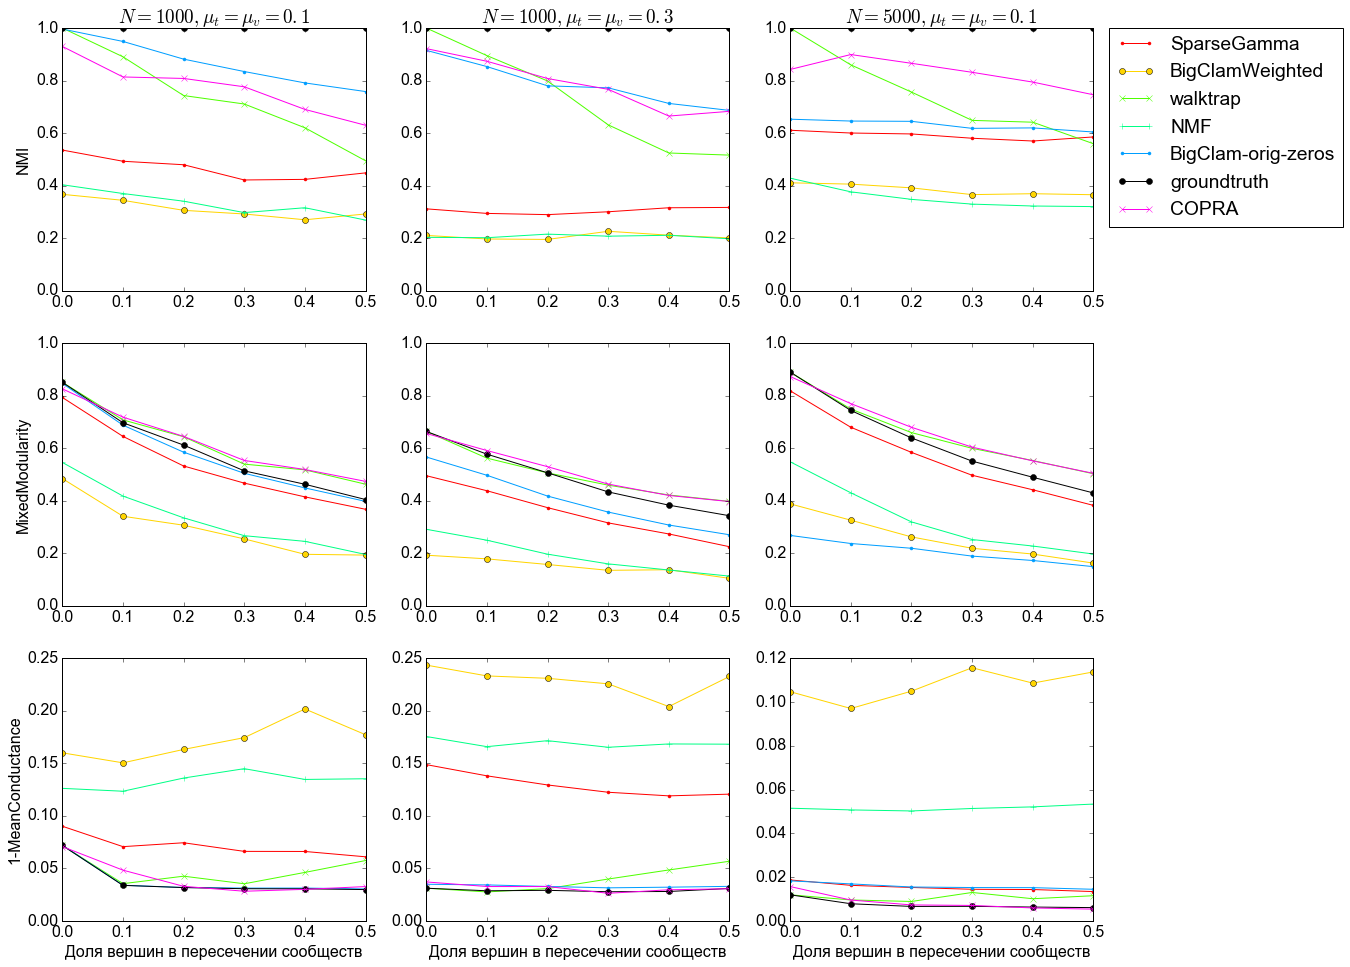
\includegraphics[width=\textwidth]{imgs/experiments_all.png}
	\caption{Результаты работы методов на модельных данных. На графиках изображена зависимость качества разбиения от параметра $\gamma$ --- доли вершин в пересекающихся участках сообществ. По столбцам указаны 4 варианта параметров, остальные параметры зафиксированы и указаны в Таблице \ref{table:bench_params}. По строкам различные метрики: NMI, MixedModularity, 1-MeanConductance (Единица минус среднее значение проводимости по всем сообществам).}
	\label{fig:experiments}
\end{figure*}

Проанализировав графики, можно заметить, что предложенные методы не лучше остальных в решении данной задачи. Лидируют такие алгоритмы как оригинальный \textit{BigClam}, \textit{COPRA}, \textit{walktrap}. Последний метод занимается поиском непересекающихся сообществ и проигрывает первым двум методам как только значение $\gamma$ отходит от нуля.
Метод \textit{SparseGamma} работает лучше, чем наивное обобщение BigClam, но хуже, чем оригинальный метод. 
Отметим, что по смешенной модулярности на больших графах BigClam проигрывает двум другим методам. 

Можно заметить интересную особенность, что такой простой метод как \textit{NMF} и наивное обобщение BigClam в данной задаче имеет подавляющее преимущество по функционалам связанными с проводимостью. Причины такого поведения не были прояснены.
При чем, как можно судить по NMI, результирующая структура сообществ получилась хуже чем у других методов. 
Скорее всего последняя метрика плохо подходит для этих данных, либо этого класса задач, так как значение истинного разбиения по этой метрике находится в самом низу графика, как и лучшие по NMI методы.

Можно предположить, что в данном модельном примере информация, которую с собой несет вес ребра, не достаточно значительна, чтобы при ее удалении ситуация ухудшалась, а предложенные модели объяснения весов на ребрах не соответствуют действительной природе данных.

\section{Результаты работы}

В работе предложен новый подход для выделения пересекающихся сообществ во взвешенных графах. 
Алгоритм является обобщением BigClam на взвешенный случай.
Метод протестирован на четырех модельных наборах данных. 
Полученные результаты говорят о том, что алгоритм работает хуже современных методов, решающих подобную задачу. 

В ходе работы предложены новые улучшенные способы инициализации на основе значения проводимости, которые позволяют ускорить существующие методы выделения пересекающихся сообществ и достичь лучших значений функционала.
Из экспериментов видно, что предложенный метод не использует всю ту информацию, которая дополнительно содержится в весах графа. 
Подход нуждается в доработке, что планируется сделать в дальнейшей работе.

\bibliographystyle{amsplain}
\bibliography{bibl}

\end{document}
